\newpage
\section{Changements de repère}
Jusqu’à présent, nous avons travaillé dans des repères dont les axes étaient alignés avec ceux des coniques considérées.
Mais que se passe-t-il lorsque le repère n’est pas orienté comme on le souhaite par rapport à la conique ?

Dans ce cas, il suffit d’effectuer un changement de repère, un changement de variables, en combinant éventuellement une translation et une rotation.

\subsection{Translation}
Pour translater un repère et recentrer le repère au point $(x_c, y_c) \neq (0,0)$, on introduit de nouvelles variables définies par :\\
$X = x - x_c$ et  $Y = y-y_c$. 

Les axes du nouveau repère sont 2 à 2 parallèles à ceux du premier repère.
\subsubsection{Ellipse}
\begin{tcolorbox}[colback=cyan!5, colframe=cyan!70!blue, title=Equation cartésienne d'une ellipse de centre {$(x_c, y_c)$} (sans rotation).]
Soit $a, c \in \mathbb{R}^+_0$ tels que $a > c$.\\
 Dans un repère orthonormé, 
 considérons une ellipse centrée en $(x_c, y_c)$ dont les foyers sont 
 $F_1 (x_c - c,y_c)$ et $F_2 (x_c+c,y_c)$ et dont le grand axe mesure $2a$.\\ Alors son équation cartésienne s'écrit\\
\begin{equation}
\mathcal{E} \equiv \dfrac{(x-x_c)^2}{a^2} + \dfrac{(y-y_c)^2}{b^2} = 1
\end{equation}
Avec $b^2 = a^2 - c^2$, $(0<b<a)$.
\end{tcolorbox}

\subsubsection{Hyperbole}
\begin{tcolorbox}[colback=cyan!5, colframe=cyan!70!blue, title=Equation cartésienne d'une hyperbole de centre {$(x_c, y_c)$} (sans rotation).]
Soit $a, c \in \mathbb{R}^+_0$ tels que $c > a$.\\
 Dans un repère orthonormé, 
 considérons une hyperbole centrée en $(x_c, y_c)$ dont les foyers sont $F_1 (x_c - c,y_c)$ et $F_2 (x_c+c,y_c)$, et dont la différence des distances à chaque foyer 
est constante et égale à $2a$.\\ Alors son équation cartésienne s'écrit\\
\begin{equation}
\mathcal{H} \equiv \dfrac{(x-x_c)^2}{a^2} - \dfrac{(y-y_c)^2}{b^2} = 1
\end{equation}
Avec $b^2 = c^2-a^2$, $(0<b<c)$.
\end{tcolorbox}


\subsection{Rotation}

Lorsque la conique est orientée de manière oblique par rapport au repère initial, \\il est possible de réaliser une rotation de repère afin d’aligner les axes du nouveau repère avec les axes de la conique.  

\begin{minipage}{0.5 \textwidth}
    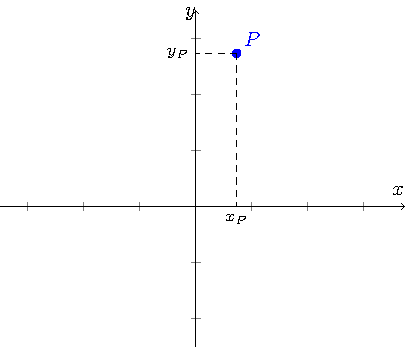
\includegraphics[scale = 0.8]{./sections/tikz_standalone/gen_rot_01.pdf}
\end{minipage}
\hfill
\begin{minipage}{0.5 \textwidth}
    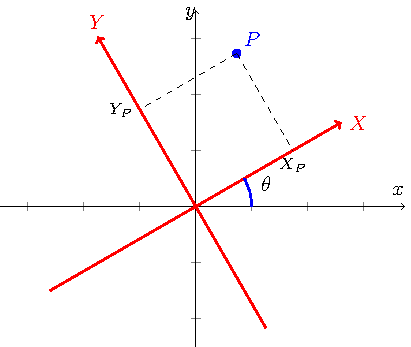
\includegraphics[scale = 0.8]{./sections/tikz_standalone/gen_rot_00.pdf}
\end{minipage}

\vspace{1cm}
\begin{minipage}{0.5 \textwidth}
    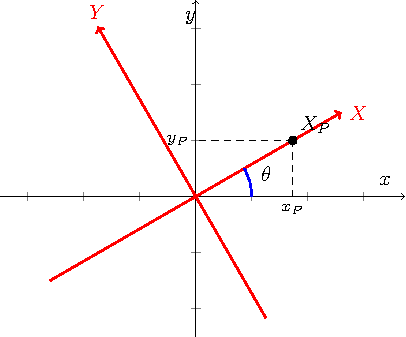
\includegraphics[scale = 1]{./sections/tikz_standalone/gen_rot_1.pdf}
\end{minipage}
\hfill
\begin{minipage}{0.5 \textwidth}
    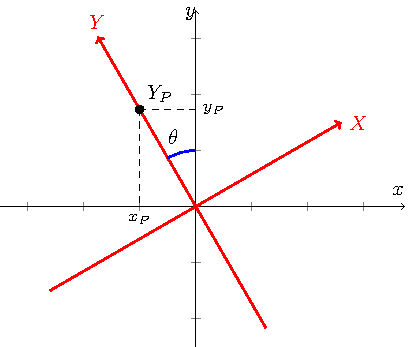
\includegraphics[scale = 1]{./sections/tikz_standalone/gen_rot_2.pdf}
\end{minipage}

Dans ce cas, les coordonnées \((x, y)\) dans le repère initial et les coordonnées \((X, Y)\) dans le repère tourné sont liées par les relations suivantes :
\[
\begin{cases}
    x = X \cos \theta - Y \sin \theta,\\[2mm]
    y = X \sin \theta + Y \cos \theta,
\end{cases}
\]
où \(\theta\) représente l’angle de rotation du repère.\\
La démonstration est laissée en exercice au lecteur.\\

Dans le cas où $\theta = \dfrac{\pi}{2}$, on a alors :
\[
\begin{cases}
    x = - Y,\\[2mm]
    y = X,
\end{cases}
\]
\subsubsection{Ellipse}
\begin{tcolorbox}[colback=cyan!5, colframe=cyan!70!blue, title=Equation cartésienne d'une ellipse de centre {$(0,0)$} avec une rotation de {$\dfrac{\pi}{2}$}.]
Soit $a, c \in \mathbb{R}^+_0$ tels que $a > c$.\\
 Dans un repère orthonormé, 
 considérons une ellipse centrée en $(0, 0)$ dont les foyers sont $F_1 (0,-c)$ et $F_2 (0,c)$ et dont le grand axe mesure $2a$, alors\\
\begin{equation}
\mathcal{E} \equiv \dfrac{x^2}{b^2} + \dfrac{y^2}{a^2} = 1
\end{equation}
Avec $b^2 = a^2 - c^2$, $(0<b<a)$.
\end{tcolorbox}

\subsubsection{Hyperbole}
\begin{tcolorbox}[colback=cyan!5, colframe=cyan!70!blue, title=Equation cartésienne d'une hyperbole de centre {$(0,0)$} avec une rotation de {$\dfrac{\pi}{2}$}.]
Soit $a, c \in \mathbb{R}^+_0$ tels que $c > a$.\\
 Dans un repère orthonormé, 
 considérons une hyperbole centrée en $(0, 0)$ dont les foyers sont $F_1 (0,-c)$ et $F_2 (0,c)$
, et dont la différence des distances à chaque foyer 
est constante et égale à $2a$.\\ Alors son équation cartésienne s'écrit :
\begin{equation}
\mathcal{E} \equiv \dfrac{x^2}{b^2} - \dfrac{y^2}{a^2} = -1
\end{equation}
Avec $b^2 = c^2 - a^2$, $(0<b<c)$.
\end{tcolorbox}

Dans ce cas, l'axe focal est l'axe y et l'axe non focal est l'axe x.

\section{Equation générale d'une conique}\label{section:generale}